% !TEX root=/home/tavant/these/manuscript/src/manuscript.tex

\section{Collisionless kinetic model and polytropic state law}
\label{sec-kinetic}


The previous section showed that the electrons are not Maxwellian, similarly to the \ac{2D} results.
In this section, we use the 1D kinetic equation in order to highlight the important phenomena needed to describe the sheath.
\subsection{Vlasov equation for the sheath}

Because the sheath is thin and the neutral pressure is low, we neglect the collisions in the sheath, so that we only need to solve Vlasov's equation.
The stationary 1D-3V Vlasov equation for the EVDF reads\string:
\begin{equation}\label{eq-vlasov}
  v_x \cdot \partial_x f_e \vec{e}_x + \frac{e}{m_e} \nabla \phi \cdot \nabla_v f_e = 0,
\end{equation}
Since the electrostatic potential depends only on $x$, \cref{eq-vlasov} becomes,
\begin{equation}
v_x \partial_x f_e +  \frac{e}{m_e}\partial_x\phi \partial_{v_x} f_e = 0
\label{eq-vlasov1D}
\end{equation}
The variables $v_y$ and $v_z$ do not play any role, such that they can be hold constant, and we can solve \cref{eq-vlasov1D} with $f_e$ as a function of $x$ and $v_x$ only.

In order to solve \cref{eq-vlasov1D} in the sheath,  we use the following boundary conditions\string:
  \begin{enumerate}
\item At the plasma sheath boundary ($x=x_s$) the EEDF is imposed\string:
\begin{equation}
f_e(x_s, v_x) = f_0(v_x),
\label{eq-plasma_BC}
\end{equation}
\item At the wall ($x=x_w$) the particles are absorbed, such that
\begin{equation}
f(x_w, v_x<0) = 0
\label{eq-wall_BC}
\end{equation}
\end{enumerate}

The partial derivative equation (\ref{eq-vlasov1D}) can be solved by the method of the characteristics. We introduce the function $\gamma(x)$ such that
\begin{equation}
\frac{df_e(x,\gamma(x))}{dx} = \partial_x f_e + \gamma' \partial_{v_x} f_e = 0
\end{equation}
Combining this equation with \cref{eq-vlasov1D} for $v_x = \gamma(x)$,
\begin{equation}
\left( \frac{e\phi'}{m_e} - \gamma \gamma' \right) \partial_{v_x} f_e = 0
\label{eq-char}
\end{equation}
In general $\partial_{v_x} f_e \neq 0$ such that $(e\phi'/m_e - \gamma\gamma')$ can be integrated
\begin{equation}
\frac{\gamma(x)^2}{2} - \frac{e\phi(x)}{m_e} = \frac{\gamma(x_s)^2}{2} - \frac{e\phi_s}{m_e}
\end{equation}
Since the EVDF is conserved along the contour $\gamma$,
\begin{equation}
f_e(x,\gamma(x)) = f_e(x_s, \gamma(x_s))
\end{equation}
and
\begin{equation}
\gamma(x_s) = \left[ \gamma(x)^2 - \frac{2e(\phi(x) - \phi_s)}{m_e} \right]^{1/2}
\end{equation}
with $\phi_s$ the plasma potential at the sheath edge.
Using \cref{eq-plasma_BC},
\begin{equation}
f_e(x,v) = f_0\left( \left[ v^2 - \frac{2e(\phi(x) - \phi_s)}{m_e} \right]^{1/2}\right)
\label{eq-sol}
\end{equation}
Condition (\ref{eq-wall_BC}) yields a condition on $f_0$\string:
\begin{equation}
\text{for all } v > \left( \frac{2e\phi_s}{m_e} \right)^{1/2}, f_0(v) = 0
\label{eq-trunc}
\end{equation}
This simple collisionless model explains rigorously how the tail of the EVDF is cut by the wall absorption.
This asymmetry of the EVDF could press us to separate the electrons into the one going toward the wall and the one going away from the wall.
\Cref{fig-EVDFpm} shows the EEPF of the electron going toward and from the wall.
We can see that there only is a small difference between the  EEPF of the two populations.
Indeed, as the domain is symmetric and bounded in the two directions, the population coming toward the wall is also depleted by the opposite wall.
Hence in the following, we will neglect this asymmetry due to the wall.


\begin{figure}[!hbtp]
  \centering
  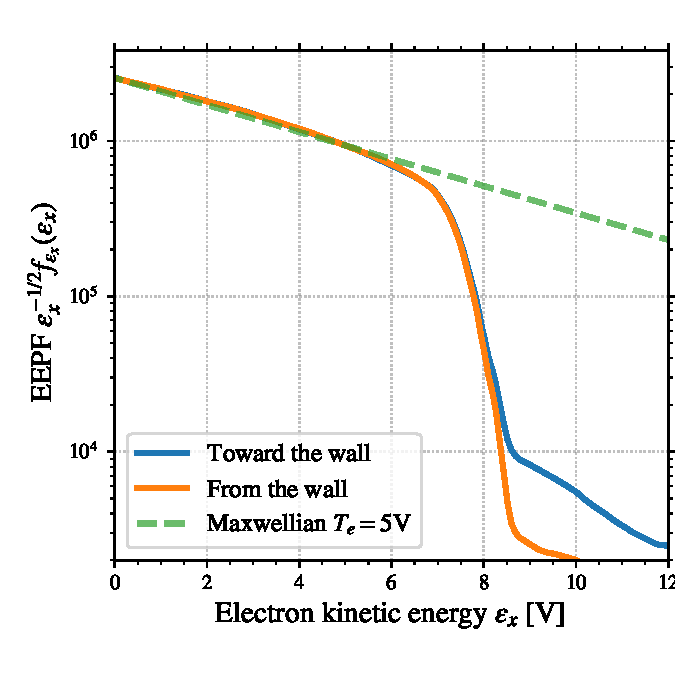
\includegraphics[width=\defaultwidth]{EVDFpm.pdf}
  \caption{EEPF measured in the PIC simulations of the electrons going toward and from the wall at $x=23.7mm$. The green dashed line corresponds to a Maxwellian distribution of 5$\eV$.}
  \label{fig-EVDFpm}
\end{figure}

\begin{figure}[!hbtp]
  \centering
  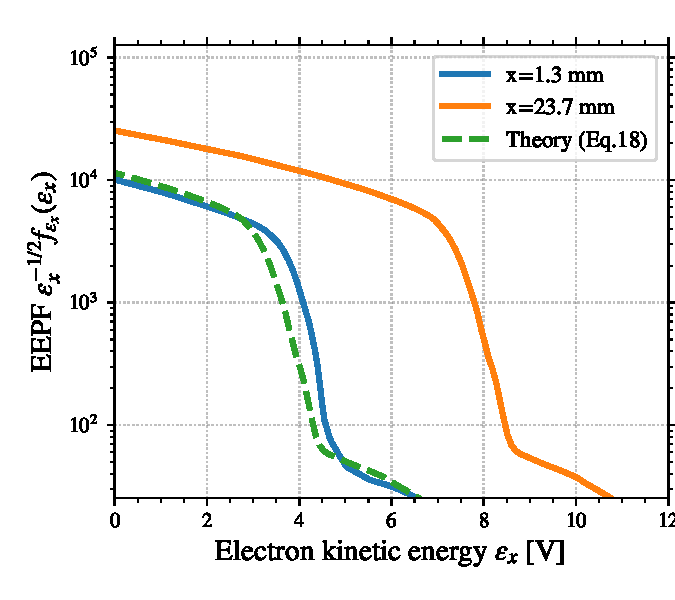
\includegraphics[width=\defaultwidth]{EVDFshift.pdf}
  \caption{Evolution of the EEPF between 1.3mm (in blue) and 23.7mm (in orange) from the wall. Is overlaid (in dashed green) the expected  EEPF at $x=1.3$mm using the EEPF at $x=23.7$mm and the potential difference in \cref{eq-sol}. }
  \label{fig-PICEEPF}
\end{figure}

\Cref{fig-PICEEPF} compares the EEPF from \cref{eq-sol} with the PIC simulation between the position $x=1.3$\,mm and $x=23.7$\,mm.
The plasma potential reads $\phi(x=1.3\,{\rm mm})=4.1$\,V and  $\phi(x=23.7\,{\rm mm})=7.7$\,V.
We can observe a very good agreement between the actual evolution of the EEPF measured in the simulations and the prediction of \cref{eq-sol}.
This confirms the possibility to neglect the collisions in the sheath.

\subsection{Polytropic state law for the electrons}

The evolution of a two-$\Te$ EEDF  in a collisionless potential drop has been studied by \citet{zhang2016}.
The authors have shown that the evolution of the electron population can be described using a polytropic index $\gamma$, such that\string:
\begin{equation}
  \label{eq-poly}
  \nabla_x \left( p_{e,x}(x) n_e(x)^{-\gamma} \right)= 0
\end{equation}
with $p_{e,x}$ the electron pressure.
The value of $\gamma$ is related to the two temperatures $T_1$ and $T_2$, and for $T_1 > T_2$, we have $\gamma > 1 $.




\begin{figure}[!htbp]
  \centering
  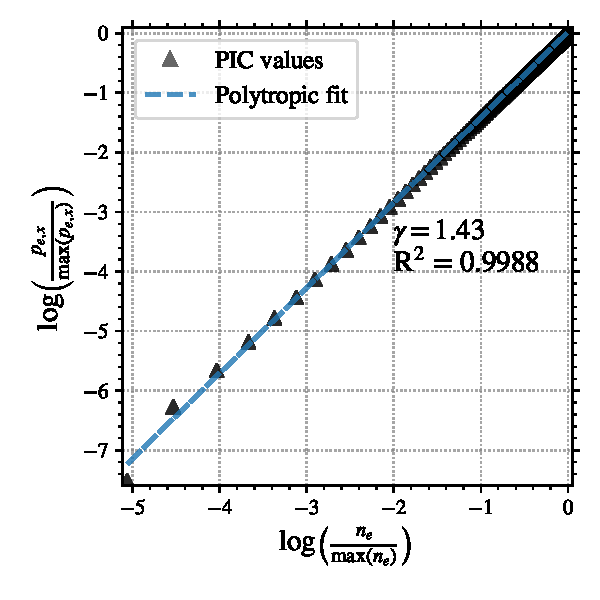
\includegraphics[width =\defaultwidth]{Polytropic.pdf}
  \caption{Electron pressure as a function of the electron density observed in the PIC simulations of \cref{fig-PIC1} (black markers), and the linear fit (blue dotted line) in order to determine $\gamma$.}
  \label{fig-polyFit}
\end{figure}

\Cref{fig-polyFit} shows the PIC simulation results presented in \cref{fig-PIC1} in log scale.
Each marker represents one cell of the PIC simulation.
Overlaid is a linear regression which slope is the polytropic index $\gamma$.
The regression is conducted over the whole simulation domain.
We can see that the linear regression fits the simulation results with a very good agreement (R$^2$ = 0.999).
The value $\gamma = 1.43$ is significantly higher than the isothermal case ($\gamma_{\rm isothermal} = 1$).
Interestingly, while the polytropic law observed in \citet{zhang2016} was only for a collisionless evolution, here the polytropic law is observed in both the collisionless sheath and the modestly collisional plasma region.

The polytropic law of \cref{eq-poly} can be used in order to close the fluid equation without the isothermal hypothesis.
The non-isothermal fluid model for the sheath is the subject of the next section.
A polytropic index for the ions has already been proposed in order to link the ions kinetics and the fluid parameters \citep{kuhn2006,jelic2007}.
The approach here is essentially the same but applied to the electrons.


\subsection{Evolution of the polytropic index}

We investigate the effect of the neutral pressure on the polytropic index $\gamma$.
We recall that the electron elastic scattering and momentum transfer are modeled, while the ionization and the heating are not self-consistent, but they are similar to the \ac{2D} \ac{PIC} models of \cref{ch-2}.
\Cref{fig-p} presents the evolution of $\gamma$ as a function of the pressure.
We can see that the polytropic index decreases from 1.7 to 1.4 as the pressure increases from 0.05 to 10 mTorr.
This is in agreement with the fact that the high energy electron population is mostly replenished by the electron-neutral scattering \cite{kaganovich2007}.
Increasing the collisions while keeping the other parameters constant provides more electrons to the high energy tail, hence reducing the polytropic index \citep{zhang2016}.

\begin{figure}[!htbp]
  \centering
  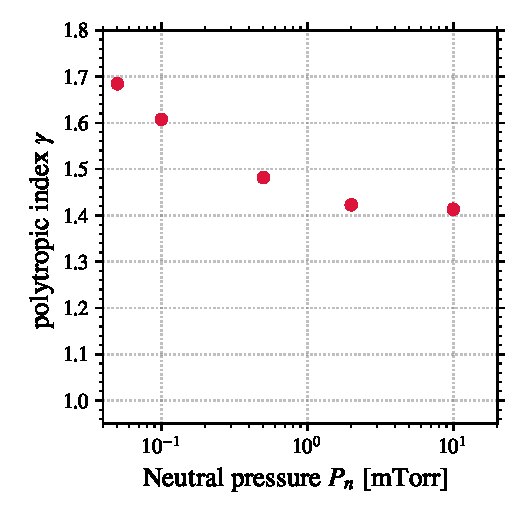
\includegraphics[width=\defaultwidth]{/pressur_effectLog.pdf}
  \caption{Effect of the background neutral pressure over the polytropic index $\gamma$ in the PIC simulations using \M1. As a reminder, the isothermal case corresponds to $\gamma=1$.}
  \label{fig-p}
\end{figure}

Other parameters are also expected to modify $\gamma$.
For instance the size of the simulation, the electron mean energy, and the nature of the gas.

\subsection{Coulomb collision and improvements}

\begin{itemize}
  \item compare the order of magnitude of coulom collision and the others
  \item Discuss about the thermalization model of Krooks (or something like that)
\end{itemize}
